\documentclass[psfig,preprint]{aastex}

\makeatletter
\renewcommand\theequation{\thesection.\arabic{equation}}
        \@addtoreset{equation}{section}
\renewcommand\thefigure{\thesection.\arabic{figure}}
        \@addtoreset{figure}{section}
\renewcommand\thetable{\thetable.\arabic{table}}
        \@addtoreset{table}{section}
\makeatother


\begin{document}

\setcounter{section}{-1}

\title{DISCREETLY FINE TIMES \\ with \\ DISCRETE FOURIER TRANSFORMS \\
(DFT's with DFT's) \\ or \\ ``WHY DOES THAT FFT OUTPUT LOOK SO
WEIRD???''}

\author{\copyright Carl Heiles \today }

          ``Spectral analysis'' means describing a time-varying signal
by its power spectrum, otherwise known as its Fourier spectrum or its
frequency spectrum.  It should be obvious that such spectra are essential for
astronomers: for example, spectra tell us not only about pulsar periods,
but also about chemical composition in stars and Doppler velocities. 
But the description of signals in terms of spectra or Fourier components
has importance in many fields, and this becomes obvious on just a little
reflection.  A prime example: a bridge is subject to shaking by
earthquakes; if its natural resonance frequency is close to the
frequency of ground movement, you've got trouble!

	Spectral analysis is an integral part of some of our labs.  We
will sample signals at regular intervals with our computers, a process
known as ``discrete sampling'', and our computers will change the
voltages to digital numbers, a process known as ``digitization''. We'll
then do a discrete Fourier transform to calculate the power spectrum.
There are some intricacies with this process\dots

\tableofcontents

\section{THE INTEGRAL FOURIER TRANSFORM: TIME $\leftrightarrow$ FREQUENCY}

\subsection{Classical Fourier transforms}

          We use the Fourier transform (FT) to convert a time-varying
voltage $E(t)$ from the time to the frequency domain $E(\nu)$, and {\it
vice versa}.  The formally correct equations are

\begin{mathletters} \label{eqone}
\begin{equation}
E(\nu) = \int_{-\infty}^{\infty} E(t) e^{[2 \pi i]\nu t}  dt \; 
\end{equation}

\noindent and, to go the other way, 

\begin{equation}
E(t) = \int_{-\infty}^{\infty} E(\nu) e^{-[2 \pi i]\nu t}  d\nu \; 
\end{equation}
\end{mathletters}

In our case, we are going to modify this a bit so that we don't run into
infinities. We will write\dots

\begin{equation} \label{eqtwo}
E(\nu) = \lim_{T \to \infty} {1 \over 2T}
\int_{-T}^{+T} E(t) e^{[2 \pi i]\nu t}  dt \; .
\end{equation}

\noindent We are often interested in the {\it power spectrum}.   Power
goes as amplitude squared, so the power spectrum $P(\nu ) \propto E(\nu
)^2$.  A small complication: $E(\nu)$ can be complex, but the power
spectrum is just watts per Hz and must be real.  We take care of this by
defining

\begin{equation}
P(\nu ) = E(\nu ) \times [E(\nu )]^* \; ,
\end{equation}

\noindent where the superscripted $[E(\nu)]^*$ means the complex
conjugate.  This multiplication is the equivalent of ``detection''. 

\section{EFFECTS OF $T$ BEING FINITE: INTEGRAL TRANSFORMS}

\label{sectiontwo}

	There's a fundamental fact of the real world: we don't live
forever, and even if we did TAC's wouldn't allow us infinite telescope
time for our precious projects, so we never can allow $T \rightarrow
\infty$.  This frustrates the old politicians who want absolute control
over everything, forever.  Less seriously in some circles---and more in
others---it has two major ramifications for Fourier transform devotees:
\begin{enumerate}

	\item It limits the frequency resolution.

	\item It produces ``spectral leakage'': The result at a given
frequency in the Fourier transform spectrum is contaminated by those at
{\it all other} frequencies in the spectrum!
\end{enumerate}

	We treat these two ramifications in the following subsections.

\subsection{Spectral Resolution} \label{spctres}

        Equations \ref{eqone} and \ref{eqtwo} are fine as they stand,
but when we sample a signal $T$ is finite. This limits our spectral
resolution. To understand this, consider the analytic solution of
equation \ref{eqtwo} for a monochromatic cosine wave of frequency
$\nu_s$, that is $E(t) = \cos(2 \pi \nu_s t)$.  For $T \rightarrow
\infty$, $E(\nu) = 0$ except for $\nu = \nu_s$; this is commonly
expressed by the term ``Dirac delta function''.  But more generally, we
have as the analytic solution

\begin{equation} \label{sinxoverx}
E(\nu) = {\sin (2 \pi (\nu - \nu_s) T) \over 2 \pi (\nu - \nu_s)
T} \; .  
\end{equation}

\noindent It is simpler to write $\delta \nu = (\nu - \nu_s)$ and write

\begin{equation}
E(\nu) = {\sin (2 \pi \delta \nu T) \over 2 \pi \delta \nu T} \; .
\end{equation}

\begin{equation}
P(\nu) = \left ({\sin (2 \pi \delta \nu T) \over 2 \pi \delta \nu T}
\right)^2 \; .
\end{equation}

\noindent and we see that this is just the famous $\sin x \over x$ type
behavior.  This quantitatively expresses the degradation in frequency
resolution when you sample for a finite time; roughly, the spectral
resolution is the width of this function, which is $\Delta \nu \sim {1
\over T}$.

	In optical and IR astronomy, the need for high spectral
resolution leads to the requirement of long time delays, which in turn
means long path lengths. For grating and prism spectrometers, this can
be achieved only by using physically large devices. For a Fabry-Perot,
the long path is achieved by multiple reflections. In terms of the
conventional definition of resolving power, ${\Delta \lambda \over
\lambda} \sim {\lambda \over size}$. There's no way around this!

\subsection{Spectral Leakage}

	Not only is the infinitesimally-narrow delta function replaced by
a function of width $\sim {1 \over 2T}$ but also the function $\sin x
\over x$ has ``sidelobes'': it spreads power out over a huge range of
frequencies, albeit---after squaring, anyway---at a low level.  The
spread-out power gets weaker as you move away from the signal, that is
as $\delta \nu$ increases---but it doesn't decrease monotonically. 
Rather, the    sidelobes mean that there the spread-out power goes to
zero periodically for $\delta \nu = {1 \over 2T}$.  In colloquial terms,
the power of the monochromatic sine wave ``leaks'' away in the power
spectrum to all frequencies.  Not surprisingly, this is called
``spectral leakage''. It's covered in NM chapter 13.4.

        You can reduce spectral leakage by using a ``window function''
$W(t)$ that is not ``square''.  What on Earth does this mean? In equation
\ref{eqtwo}, when you use a finite $T$ you are integrating over a    
``window'' of total length $2T$, as follows:

\begin{equation}
E(\nu) = {1 \over 2T}
\int_{-T}^{+T} W(t) E(t) e^{[2 \pi i]\nu t}  dt \; .
\end{equation}

\noindent In equation \ref{eqtwo}, the window function $W(t)$ is unity;
when  we let $W(t) = 1$ for the time window of length $2T$, then this is
called a ``square window function''.  A square window function produces 
``sharp edges'' in the sense that the function $E(t)$ has its full
amplitude for all $t$ within the window and then cuts off precipitously
at the ends of the window.  {\it It's this sudden cutoff---the sharp
edge---that produces spectral leakage.}

        We can reduce spectral leakage by making $W(t)$ a function that
produces a {\it gradual} cutoff so as to eliminate the sharp edge.  We
make $W(t)$ a function that gradually falls to zero at the window edges
$-T$ and $T$. As one possible example among many, consider the Hanning
weighting function, which is commonly used in radio astronomy:

\begin{equation}
W(t) = {1 \over 2} \left( 1 + \cos{\pi t \over T} \right) \; .
\label{weighting}
\end{equation}

\noindent This drastically reduces the sidelobes.  This comes at a
price, though: the spectral resolution gets worse---by about a factor
of two.  The reason is that the window function $W(t)$ goes to zero
at the ends of the time window $2T$, which effectively makes the window
shorter. {\it Note:} We also use the term ``weighting function'' for
$W(t)$.



\section{DISCRETELY SAMPLED SIGNALS}

	When I was a teenager we had vinyl records.  They contained {\it
continuously-sampled} signals that were directly imprinted on the vinyl. 
Today we focus on CD's.  These contain {\it discretely-sampled} signals
that are digitized and written on to the little silver disk.  The fact
that CD's contain discretely sampled data means that the signal is known
only for certain specific times.  In particular, the signal is not
sampled {\it between} these times.  Does this mean that CD's don't sound
as good as the vinyl records?

	Regarding the calculation of our power spectrum with a FT, you'd
think that the replacement of an integral by a sum would be
straightforward, with no subtleties.  But this {\it isn't the case}. 
There {\it are} subtleties, and they are {\it crucial}.  Understanding
them, and dealing with them properly, makes your CD's sound just as good
as vinyl.  So read on: we'll first provide a qualitative introduction
and then go into details.

\subsection {Discretely-Sampled Signals: The Nyquist Criterion.}

	When your CD music is recorded, or in astronomy when we observe
a pulsar or sample an incoming signal to determine the spectrum, we
sample the incoming signal sequentially in time, at regular intervals
called the {\it sampling interval} $\Delta t = t_{smpl}$.  Equivalently,
we are sampling at a regular rate called the sampling frequency
$\nu_{smpl} = {1 \over t_{smpl}}$. 

	In discrete sampling, we first require that the signal be
limited in bandwidth.  That is, the highest frequency in its spectrum
must be limited to an upper cutoff, which we call the bandwidth $B$;
thus, the frequencies in the signal extend from 0 to $B$ Hz.  Then we
must sample the signal periodically at a fast enough
rate---specifically, we require ($\nu_{smpl} \ge 2 B$ Hz).  This is the
``Nyquist criterion''.  If the Nyquist criterion is violated, we have
the problem of {\it aliasing}, which means that signals with frequencies
$\nu > B$ {\it appear} as {\it lower} frequencies.  Remember those
movies showing cars and the wheels that seem to rotate backwards? That's
a real-world example of aliasing: the movie frames discretely sample the
scene at too slow a rate to faithfully reproduce the wheel's rotation. 
You can understand aliasing by looking at Figure \ref{figone}. 

\begin{figure}[!h]
\begin{center}
\leavevmode
%\includegraphics[scale=.55, angle=90]{lsfitfig.ps}
\includegraphics{fig1.ps}
\end{center}

\caption{Aliasing at its worst. The sample interval is $t_{smpl}= 0.01$
s, so the sample frequency is $\nu_{smpl} = 100$ Hz. The Nyquist
frequency is $f_N=50$ Hz. The stars are the datapoints. The two signals
shown are at frequencies 37.5 and 62.5, i.e.\ $f_N \pm 12.5$ Hz. Which
signal do the datapoints represent? \label{figone} }
\end{figure}

	To put it another way: When we sample at rate $\nu_{smpl}$, the
maximum signal frequency that can be faithfully reproduced is
$\nu_{smpl} \over 2$.  This is called the Nyquist frequency and here we
denote this by $f_N = {\nu_{smpl} \over 2}$.  Clearly, the signal's
bandwidth $B$ must satisfy $B \le f_N$. All this is called the {\it
sampling theorem}.

	How rapidly must music be sampled for recording on a CD? The
human ear responds to something like 20 kHz.  To prevent aliasing, we
need to sample at twice this, at about 40 kHz. 

\subsection {A Popular MISCONCEPTION!!!}

	Somebody, sometime, will probably tell you that aliasing has to
do with {\it discrete Fourier transforms}.  Tell them to go jump in the
lake.  It has to do with the sampling rate.  Period.  Aliasing occurs if
you don't sample fast enough, and affects your results {\it whether or
not} you are dealing with Fourier transforms.  If you don't believe me,
just look again at Figure \ref{figone}. And remember what happens to rotating
wheels in movies. 

\section{DISCRETE SAMPLING AND THE FOURIER TRANSFORM}

          We use the Fourier transform to convert from the time to the
frequency domain, and {\it vice versa}.  For continuously-sampled
signals we use the Fourier integral, equation \ref{eqtwo}. For
discretely-sampled signals we have to replace this by a summation.  This
is the {\it discrete Fourier transform}, or DFT. 

\subsection {The maximum recoverable bandwidth: the Nyquist frequency}

         OK, we've sampled our signal at regular intervals $t_{smpl}$,
meaning that the sampling frequency is $\nu_{smpl} = {1 \over t_{smpl}}$
and $f_N = {\nu_{smpl} \over 2}$. If we do this for time $2T$ then we
obtain $2J = {2T \over t_{smpl}}$ independent points. From these we wish
to compute the spectrum.

	If we want to digitally compute the Fourier transform, then the
first thing we  must realize that the original $2J$ channels provide
only $J$ spectral points! This seems like a loss of information, but
it's not: the spectrum is {\it complex}, so those $J$ complex numbers
contain $2J$ independent numbers. 

	With sample frequency $\nu_{smpl}$ we obtain the spectrum for
the range of frequencies $0 \rightarrow {\nu_{smpl} \over 2}$ or $0
\rightarrow f_N$; this is known as the {\it bandwidth}, denoted by $B$.
With $J$ independent points, the separation (and the frequency
resolution) is $\Delta \nu = {\nu_{smpl} \over 2J}$. Fortunately,
${\nu_{smpl} \over 2J} = {1 \over 2 J t_{smpl}} = {1 \over 2T}$; this
confirms our earlier discussion in \S \ref{spctres} about frequency
resolution. 

	But more importantly for the present discussion, when sampling
at rate $\nu_{smpl}$ you cannot recover a spectrum wider in bandwidth
than $f_N = {\nu_{smpl} \over 2}$. 

	Amazingly, a discretly sampled time series occurs where you'd
least expect it: in a common, garden-variety optical analog device,
namely the classical optical grating spectrometer. The incoming light
strikes the grating at angle $\theta$ away from the normal and for the
first order reflection leaves at the same angle. Thus the difference in
time delay from one groove to the next is ${2s \cos \theta \over c}$,
where $s$ is the groove separation. You don't have any information for
time differences between these values. So this is exactly equivalent to
$t_{smpl}$, so the maximum fractional bandwidth is ${f_N \over f} = {1
\over 4 {s \over \lambda} \cos \theta}$. To attain a substantial
fractional bandwidth, e.g.\ ${f_N \over f} > {1/2}$ say, we require the
spacing $s < {\lambda /2 \cos \theta}$. Moreover, to avoid aliasing it's
absolutely necessary to insert a filter in front of the grating to limit
the input bandwidth. 

\subsection {Summary: The Two Fundamental Parameters in Discrete
Sampling and Fourier Transforms}

	The above two parameters are the fundamental ones.  

	{\bf (1)} To prevent aliasing, we must satisfy the sampling
theorem: the total signal bandwidth $B$ must be small enough , so $B
\leq f_N$, or $B \leq {\nu_{smpl} \over 2}$.\footnote{For complex input,
which can occur in radio astronomy and some other applications, the
discussion becomes more interesting.} Usually you need to limit the
bandwidth with a filter.

	{\bf (2)} In the Fourier-transformed power spectrum, the spectral
resolution is the reciprocal of the total time over which the FT is
computed: $\Delta \nu ={1 \over T_{tot}}$. 

\section{THE DISCRETE FOURIER TRANSFORM AND DISCRETE SAMPLING}

\label{four}

	With the DFT, we have to replace the Fourier integral in
equation \ref{eqtwo} by a summation.  Let's do this with a one-to-one
correspondence of the terms. First we rewrite equation \ref{eqtwo} to
make it easier for a direct comparison:

\begin{equation} \label{eqtwoa}
E(\nu) = {1 \over 2T}
\int_{-T}^{+T} E(t) e^{[2 \pi i]\nu t}  dt \; .
\end{equation}

	In our discretely-sampled case we can replace $t$ by $j
t_{smpl}$, defined for $j = -J \rightarrow J$; $\nu$ by ${k\nu_{smpl}
\over 2J}$; and $dt$ by $t_{smpl}$.  We would calculate
$E({k\nu_{smpl}\over 2J})$ for $k = -J \rightarrow J$, so the summation
looks like\dots

\begin{equation} \label{eqfivea}
E({k\nu_{smpl} \over 2J}) = {1 \over 2Jt_{smpl}} \sum_{j=-J}^{J-1}  E(j
t_{smpl}) e^{[2 \pi i] \nu_{smpl}t_{smpl} {jk \over 2J}} t_{smpl} \; .
\end{equation}

\noindent Here we've taken $dt = \Delta t = t_{smpl} \Delta j =
t_{smpl}$ (i.e., $\Delta j=1$).  The product $t_{smpl}\nu_{smpl} = 1$,
so we can simplify our notation by eliminating these variables,
replacing ${k\nu_{smpl} \over 2J}$ by the much simpler $k$, and
replacing $j t_{smpl}$ by just $j$ and writing\dots

\begin{equation} \label{five}
E(k) = {1 \over 2J} \sum_{j=-J}^{J-1} E(j) e^{[2\pi i]
{kj \over 2J}} \; .  \end{equation}

\subsection{IMPORTANT DETAIL Regarding Limits of Summation and
Periodicities}

          Are you paying attention? If so, you should be asking why the
upper limit in equation \ref{five} on the sum is $J-1$ instead of $J$.  

	One reason is that a sum from $-J \rightarrow J$ has $(2J+1)$
samples.  But we have only $2J$ samples.  So we can't possibly sum from
$-J \rightarrow J$. 

	This doesn't matter at all.  To begin with, look at equation
\ref{five} carefully: you can verify for yourself that the trig
portion---that is, the $e^{2[\pi i] {kj \over 2J}}$ term---is {\it
periodic} in both $j$ and $k$, with period $2J$.  That is, you can use
either $k$ or $(k + 2J)$---you'll get the same answer.  Same with
$j$.\footnote{With the qualification that $k$ is an integer, i.e.\ that
you are calculating the result only for integral multiples of
$\nu_{smpl} \over 2J$. We discuss this in more detail below.}  And one
other thing: the discrete Fourier transform makes the implicit,
intrinsic, completely irrevocable {\it assumption} that the input signal
$E(j)$ is {\it also} periodic with period $2J$.  Thus the {\it entire
quantity being summed} is periodic with period $2J$.  This means, also,
that the {\it result} of the summation, namely $E(k)$, is {\it also}
periodic with period $2J$. The intrinsic, irrevocable assumption that
$E(j)$ is periodic means that we only need to know $2J$ values of
$E(j)$; the $j = 2J$ value is equal to the $j=0$ value.  

	Now, everybody knows\footnote{If you don't believe me, go look
at your elementary calculus book, in the chapter where integration was
introduced.} that when we replace an integral by a digital summation we
regard each sample as centered on a bin of width $unity \times \Delta
t$.  However, the samples at the end, with $j=-J$ and $j=J$, must have
bins of width ${1 \over 2} \times \Delta t$, so we're supposed to
include both $E(-J)$ and $E(J)$ in the sum, each with a weight of $1
\over 2$.  But because of the $2J$ periodicity, we can instead include
just one and use a weight of unity. 

	The fact that $E(j)$ is periodic with period $2J$ allows
equation \ref{five} to be written in its more conventional form

\begin{equation} \label{eqnconventional}
E(k) = {1 \over 2J} \sum_{j=0}^{2J-1} E(j) e^{[2\pi i]
{kj \over 2J}} \; \; {\rm or} \; \;
E(k) = {1 \over N} \sum_{n=0}^{N-1} E(n) e^{[2\pi i]
{kn \over N}} \ .  \end{equation}

\noindent However, this form is valid only for integral values of $k$;
see \S \ref{sectionseven}. 

\subsection{ Again: The Periodic Nature of the Discrete FT}

	Above we discussed the periodic nature of both $E(j)$ and
$E(k)$. Let's delve deeper. 

         By its very nature, the Fourier transform wants to integrate to
$\infty$. But the input signal doesn't go on forever! We have to resolve
this basic incompatibility: the input signal is sampled for a finite
time, but the Fourier transform needs it to go on forever. 

	There's only one way to resolve this incompatibility: we must
assume that the input signal {\it does} go on forever, and because we
don't know what happens outside the sampling interval $-J \rightarrow
J$, the only sensible thing to do is to assume that the input signal is
{\it periodic} with period $2J$.\footnote{You might be surprised: why
not assume the signal is {\it zero} outside the interval? {\it Answer}:
most signals don't stop simply because we stop sampling them---for
example, a pulsar. {\it More Fundamental Answer}: the math requires this
assumption!}

	This assumption of ``forever'', together with the associated
$2J$ periodicity, leads to the necessary {\it result} that the spectrum
$E(k)$ and its power spectrum $P(k) = E(k) \times [E(k)]^*$ {\it also}
go on forever, $k = -\infty \rightarrow +\infty$, and are periodic with
period $2J$. 

	Because of these periodicities, we gain complete information on
the spectrum by restricting our attention to {\it windows} of length
$2J$: these windows are the finite intervals in $(j, k)$ between the
dotted lines in figure \ref{figtwo}.  They can begin and end
anywhere---all that matters is that their length is $2J$. 


\section{THAT WEIRD-LOOKING POWER SPECTRUM---IT'S JUST A MATTER OF 
STANDARD CONVENTION}

          Above we let the indices $j$ and $k$ run from $-J \rightarrow
J-1$.  But in the real world of numerical computing, we don't use
negative indices.  You might think that the reasonable way to handle
this would be to displace the whole set of $2J$ values of $E(j)$ and
$E(k)$ upwards by $J$ so that the indices run from $0 \rightarrow 2J-1$
(this would be perfectly compatible with IDL's indexing scheme).  But
this would put the $t=0$ or $f=0$ point out in the middle, at $j$ or
$k=J$, and this isn't very convenient for lots of reasons. 

          Instead, realize that the FT is periodic in $j$ with period
$2J$.  Therefore, in equation \ref{eqfivea} it doesn't matter whether you sum from
$j = -J \to J-1$, from $j = 0 \to 2J-1$, or even (god forbid!) from $j =
-3J + 7 \to -J + 6$.  So we might as well just sum from $j = 0 \to 2J-1$
and not displace anything at all.  {\it This is the standard convention,
and it leads to the standard way in which FT arrays are stored in
memory}---not just in IDL but in just about {\it every} software
package.  It has the great advantage that the $t=0$ or $f=0$ point is
the first one in the array. 

          Above we were discussing ``the FT array'', without specifying
whether it was the input or output array.  The arrangement for the {\it
input array} works in exactly the same way as that for the {\it output}
array.  And it doesn't matter whether the independent variable for the
array is time or frequency.  {\it All FT arrays, whether input or output
and no matter what the independent variable, are arranged {\it
identically} with respect to the negative and positive values}. 

\subsection{ Enough Preaching! Let's Try an Example in IDL}

	Here we take an example with $J=32$, with the discretely-sampled
input signal being the sum of three cosine waves: $E(j) = \cos(\pi {8j
\over 32}) + 0.5[\cos(\pi {7j \over 32}) + \cos(\pi {9j \over 32})]$. 
Thus we have power at three frequencies: $k=7, 8, 9$.  There is twice as
much voltage, thus four times the power at $k=8$ than there is at $k=7,
9$.  The power spectrum consists of these three nonzero points, plus a
bunch of zeros at all other frequencies.

\begin{figure}[p!]
\begin{center}
\leavevmode
%\includegraphics[scale=.55, angle=90]{lsfitfig.ps}
\includegraphics[width=6.0in]{fourierbfig.ps}
\end{center}
\caption{Upper plots in Figs A and B show a 64-point time series and
power spectrum. Lower plots show a portion of an infinitely-long
periodic time series and power spectrum from which the 64-point ones are
extracted. \label{figtwo} }
\end{figure}

	In IDL, we denote $E(j)$ by {\bf EJ} and generate this
64-element array with the statements\dots

\begin{mathletters} 
\begin{equation} 
\bf{ EJ = cos( !pi * 8 * findgen(64)/32) }
\end{equation} 
\begin{equation} 
\bf{ EJ = EJ + 0.5*cos( !pi * 7
* findgen(64)/32) + cos( !pi * 9 * findgen(64)/32) ) }
\end{equation}
\end{mathletters}

\noindent Figure \ref{figtwo} (top) shows the plot of the 64-element
array {\bf EJ}, with the 64 crosses marking the computed points (or, in
our parlance, the discretely-sampled points).  The interference of the
sine waves makes the sampled signal look like a wave packet of frequency
$k=8$, attenuated at the middle of the time interval where $j \sim 32$. 

	The signal $E(j)$ must be periodic with period $2J = 64$ and it
must go on forever.  Figure \ref{figtwo} (bottom) shows this for a
larger slice of time in which $j = -128 \rightarrow 128$.  Our points
are computed for IDL indices $0 \rightarrow 63$; this window is shown by
the dotted lines on Figure \ref{figtwo} (bottom). 

	We take the Fourier transform [$E(k) = FT( E(j))$].  In IDL, we
denote $E(k)$ by {\bf EK} and use IDL's Fast Fourier Transform (FFT)
procedure\dots

\begin{mathletters}
\begin{equation}
{\bf EK = fft(EJ)}
\end{equation}

\noindent and get then the power spectrum $P(k)$ ({\bf PK} in IDL)\dots

\begin{equation}
{\bf PK = float(EK * conj(EK))}
\end{equation}
\end{mathletters}

\noindent For convenience, we use the {\bf float} to discard the
imaginary portion of the product, which is zero---this makes {\bf PK}
real, so that in later operations we don't have to deal with a complex
array (e.g., to plot the power spectrum we can type {\bf plot, PK}
instead of {\bf plot, float(PK)}). 

	Figure \ref{figthree} (top) shows the plot of the 64-element
array {\bf PK}, with the 64 crosses marking the computed points returned
by IDL.  The {\it positive} frequencies lie in the IDL index range $1
\rightarrow 32$ and the {\it negative} ones in the range $32 \rightarrow
63$.  As expected, there is nonzero power at only three positive
frequencies, the ones with IDL indices 7, 8, 9.  There is also power at
the three corresponding negative frequencies, the ones with IDL indices
55, 56, 57. 

	The power spectrum must be periodic with period $2J = 64$ and it
must go on forever.  Figure \ref{figthree} (bottom) shows this for a
larger slice of frequency in which $k = -128 \rightarrow 128$.  IDL
indices for {\bf PK} are $0 \rightarrow 63$; this window is shown by the
dotted lines on Figure \ref{figthree} (bottom). 

\subsection{ Is this weirdness perfectly clear? }

\label{clear}

	Probably not.  So, in the following two subsections we go
through this again in excruciating detail.  We provide first a detailed
verbal description of the arrangement, and then the shortest of short
numerical examples.  In the verbal description we focus on the output
array to make things specific, but we just as well could have focused
on the input array and replaced the word ``frequency'' by ``time''.  As
you'll see, this leads to something surprising\dots we'll discuss it
explicitly (\ref{noncontinuous}).

\subsubsection{Verbal Description}

	Again, we let the time for $E(t)$ run from $t = -T \rightarrow
+T$, with $T = J t_{smpl}$.  The corresponding frequencies run from $f =
-f_N \rightarrow +f_N$, with $f_N = {\nu_{smpl} \over 2}$. 

          All FT arrays are arranged so that the {\it first} $J+1$
channels contain the {\it positive-frequency} portion of the transform. 
Again, here we focus on the output array.  Thus, for channel $k = 0
\rightarrow J$ the frequency of channel $k$ is $\nu _k = +{k f_N \over
J}$.  Thus, channel 0 contains the $\nu =0$ result, channel 1 the $\nu =
+{f_N \over J}$ result, \dots, up to channel $J$ which contains the
maximum frequency $\nu = +f_N$. 

          The remaining $J-1$ channels contain the {\it
negative-frequency} portion of the transform.  As we go from channel $J$
to $J+1$ we would go to the next highest {\it positive}-frequency point;
but because the FT is periodic with period $2J$, this must be identical
to the corresponding point at {\it negative} frequency.  This means that
channel $J$ contains {\it not only} the result for $\nu = +f_N$, but {\it
also} the result for $\nu = -f_N$.  And the remaining $J-1$ higher
channels contain the rest of the {\it negative}-frequency points, so for
$k = J \rightarrow (2J-1)$ the frequency is $\nu _k = -f_N + {(k - J) f_N
\over J}$.  Thus channel $J$ has $\nu = -f_N$, channel $(J+1)$ has $\nu =
-f_N + {f_N \over J}$, \dots, and channel $(2J-1)$ has the $\nu = -{f_N
\over J}$ result.  If you were to consider channel number $2J$ it would
contain the next highest frequency, which is $\nu = 0$; of course, this
is identical to the result in channel 0. 

          Note that frequency can {\it always be considered to increase
with channel number}: you can even regard the big backwards jump from
$+f_N$ to $-f_N$ at channel $J$ as {\it not} being a jump because the
periodic nature of the transform means that the results for these two
frequencies must be identical, and successively higher negative
frequencies are equivalent to successively higher positive frequencies
above $+f_N$. 

          So any FT array, for example the spectrum, contains $2J$
independent points.  More generally, the FT spectrum could contain $4J$
points, or $6J$ points, etc.  We could calculate as many points as we
wish.  However, because the FT is periodic, with period $2J$, channel
$2J+1$ would contain the same result as in channel 1, etc.  So there is
no sense in calculating more than $2J$ points, because the calculations
would be redundant. 

\subsubsection{An Example}

          Consider a simple case with $J=4$; you've taken 8 time
samples.  Then the proper way to arrange the input to the FT is the
following, where the {\it left-hand matrix contains the IDL indices} and
the {\it right hand the times or frequencies}:

\begin{mathletters} \label{eqeg}
\begin{eqnarray} 
\left[
\begin{array}{r} 
0 \\ 1 \\ 2 \\ 3 \\ 4 \\ 5 \\ 6 \\ 7 
\end{array} \right] \leftrightarrow
\left[
\begin{array}{r} 
0 \times {T \over J} \\
1 \times {T \over J} \\
2 \times {T \over J} \\
3 \times {T \over J} \\
\pm 4 \times {T \over J} \\
-3 \times {T \over J} \\
-2 \times {T \over J} \\
-1 \times {T \over J} \\
\end{array} \right] 
\end{eqnarray}

\noindent and the output looks like

\begin{eqnarray} 
\left[
\begin{array}{r} 
0 \\ 1 \\ 2 \\ 3 \\ 4 \\ 5 \\ 6 \\ 7
\end{array} \right] \leftrightarrow
\left[
\begin{array}{r} 
0 \times {f_N \over J} \\
1 \times {f_N \over J} \\
2 \times {f_N \over J} \\
3 \times {f_N \over J} \\
\pm 4 \times {f_N \over J} \\
-3 \times {f_N \over J} \\
-2 \times {f_N \over J} \\
-1 \times {f_N \over J} \\
\end{array} \right] 
\end{eqnarray}
\end{mathletters}

\begin{figure}[h!]
\begin{center}
\leavevmode
%\includegraphics[scale=.55, angle=90]{lsfitfig.ps}
\includegraphics[width=4.0in]{ftfig1.ps}
\end{center}
\caption{Envisioning the window as a circle makes the relationship
between negative and positive frequencies or times. The numbers are the
multipliers of the times and frequencies in equations \ref{eqeg}.
\label{ftfig1} }
\end{figure}

\enlargethispage{0.4in}
\noindent We have been envisioning the FT array in linear space. 
However, the DFT is composed of trig functions restricted to a given
range in frequency and time.  It's helpful to step back and change our
view from linear space to {\it circular} space---to get back to
fundamentals and recall that trig functions are defined on the {\it
circle}.  As pictured explicitly in Figure \ref{ftfig1}, negative and
positive frequencies, and repeated windows, simply correspond to going
around the circle more than once, or in the opposite direction.

\subsubsection{Wait a Minute! You Mean the TIME Isn't CONTINUOUS?}

\label{noncontinuous}

	Above we said---and we meant it---that in our verbal description
we focused on {\it frequency}, but we could just as well have focused
on {\it time}. And in equation \ref{eqeg} above, where we explicitly listed
the time versus the IDL index, the time {\it begins} at $0$ for IDL
index 0, runs up to $3 \times {T \over J}$ for IDL index $3$,
and then ``wraps around'' to {\it negative} times for IDL index $\ge 4$.
So it seems that time versus IDL index is discontinuous---just like
frequency. 

	{\it Yes it's true!!} If you take a bunch of time samples and
compute the FT, you should put the negative time samples into the upper
index ranges. 

	But for the calculation of just the power spectrum, it doesn't
matter whether you bother with this reshuffling or not---you get the
same answer whether or not you reshuffle.  What it {\it does} matter for
is the cases for which you are really interested in the {\it phase} of
the FT output array.  Remember that the output array $E(k)$ in equation
\ref{eqfivea} is complex; the ratio of imaginary to real parts gives the
phase of the signal.  This phase is defined with respect to $t=0$.  If
you want the phase to be correctly defined, and if you want to regard
the samples as extending from $-T \rightarrow T$ instead of $0
\rightarrow 2T$, then you must reshuffle the discrete time samples
according to the above prescription. 

	Of course, the power spectrum doesn't have any phase
information: it's only a specification of the power versus frequency. 
In other words, detected signals have no phase information.  In our lab
work we generally don't care about the absolute phase of the signal, so
you have no need to carry out the index reshuffling before computing the
FT. 

\section{THE SPECTRUM AT AN ARBITRARY FREQUENCY}

	Equation \ref{five} provides results for discretely-spaced
frequencies at intervals $\Delta \nu = {\nu_{smpl} \over 2J}$. It's
often nice to have results for arbitrary frequencies. One way is the
brute-force approach  of equation \ref{eqfivea}, which we repeat here in
slightly modified form:

\begin{equation} \label{eqfiveb}
E({\kappa \nu_{smpl} \over 2J}) = {1 \over 2J} \sum_{j=-J}^{J-1}  E(j)
e^{[2 \pi i] {j\kappa \over 2J} } \; .
\end{equation}

\noindent Here we have eliminated $t_{smpl}$ and $\nu_{smpl}$ on the
right hand side and replaced $k$ by $\kappa$ to emphasize the fact that
$\kappa$ can be a non-integer. (For non-integral $k$, you {\it must}
carry the sum from $(-J \rightarrow J-1)$ and not $(0 \rightarrow
2J-1)$; see \S \ref{sectionseven}). 

	This is fine as long as you don't want to compute a lot of
frequencies. However, suppose you want to create four interpolated
points per original point so that you have a good visual representation
of the spectrum. Each point requires $\sim 2J$ operations, so this can
be a lot of computing.

	Instead of calculating the points from the whole time series,
you can interpolate using the spectral points themselves. In principle,
you need to include {\it all} points when computing these
interpolations.  For uniform weighting, the proper interpolation formula
in the frequency domain is (Brault \& White)

\begin{equation} \label{bw}
E(\nu) = {1 \over 2J} \sum_{j=0}^{2J-1} E(j) 
  { \sin[ \pi (\nu - \nu_j) (2Jt_{smpl})] \over
    \tan[ \pi (\nu - \nu_j) t_{smpl} ] }
\end{equation}

\noindent Note that $(2Jt_{smpl}) = 2T =$ the total time; many texts use
$T$ as the total time.

	If you are willing to live with approximate results, then you
can save a lot of computer time by including just a few original data
points on each side of the point you're calculating because most of the
contribution comes from those nearby points. For example, a good
approximation is 

\begin{equation} \label{srk}
E(\nu) = \sum_{j_{nearby}} E(j) 
  { \sin[ \pi (\nu - \nu_j) (2T) ] \over
     \pi (\nu - \nu_j) (2T)  }
\end{equation}

\noindent where $j_{nearby}$ is a set of nearby frequencies in the
original spectrum chosen as a compromise between accuracy and speed.
This equation makes sense: you are weighting the spectral points in
proportion to their sidelobe response in equation \ref{sinxoverx}. 
Restricting $j_{nearby}$ to the nearest few spectral channels to $\nu$
is sufficient for many purposes. 

	{\it Note:} Strange as it may seem, the denominators in
equations \ref{bw} and \ref{srk} are written correctly.

\subsection{Two examples}

	We consider two examples. Both have 64 datapoints; note that $64
= 2^6$.

\begin{figure}[h!]
\begin{center}
\leavevmode
%\includegraphics[scale=.55, angle=90]{lsfitfig.ps}
\includegraphics{fig3.ps}
\end{center}

\caption{Monochromatic signals with frequency 12.5 Hz (top) and 10.0 Hz
(bottom). The sample interval is $t_{smpl}= 0.01$ s, so the sample
frequency is $\nu_{smpl} = 100$ Hz and the Nyquist frequency is $f_N=50$
Hz. Stars are from the FFT, located at frequencies $(-f_N + k \Delta
\nu)$ [$\Delta \nu= {1 \over 2T}$]; the solid curve joins much more
closely spaced points calculated using equation \ref{eqfiveb}. 
\label{figthree}} \end{figure}

\subsubsection{The first example: a spike centered on integral $k$}

	First, the example of $[E(j) = \cos(2 \pi {\nu_{smpl} \over 8}
t)]$. This is a monochromatic wave whose frequency is exactly
one-quarter the Nyquist frequency, i.e.\ when plotted it is exactly
one-quarter the way between 0 and $f_N$. It falls {\it exactly} on an
integral  value of $k$. We show the resulting $E({k \nu_{smpl} \over
2J})$ by the stars in Figure \ref{figthree} (top), and we show the
almost-continuous curve from fractional values of $\kappa$ in equation
\ref{eqfiveb} as the solid curve. The stars are nonzero {\it only} for
one single value of $k$. This is because the signal frequency is {\it
exactly centered} on the frequency represented by this value of $k$. 

	But look at the solid curve. You might have thought that this
would be {\it symmetric} about the signal frequency; this is what the
analytic equation \ref{sinxoverx} seems to suggest. {\it But it's not
symmetric.} The reason is that, because the signal is real, the spectrum
is Hermetian. Hermetian means that the negative frequency real part is
equal to the positive frequency real part. (In this case, the signal is
symmetric in time, so the imaginary components are zero.) The sidelobes
of the negative frequency part interfere with those of the positive
frequency part, which causes the asymmetry. If you include the negative
frequencies in the analytic calculation, then you also find that the
sidelobes are not symmetric. 

	Similar asymmetries in sidelobe structure occur in the high end
of the spectrum because of aliasing: The sidelobes of the $\sin x \over
x$ function go on forever, so they exist at frequencies {\it beyond the
Nyquist frequency}. They are aliased back into the displayed spectrum
and this also produces asymmetry.

\subsubsection{The second example: a spike {\it not} centered on
integral $k$}

	Second, the example of $[E(j) = \cos(2 \pi {\nu_{smpl} \over 10}
t)]$. This is a monochromatic wave whose frequency is exactly one-tenth
the Nyquist frequency, i.e.\ when plotted it is exactly one-fifth the
way between 0 and $f_N$. But, in contrast to the previous example, it
does {\it not} fall on an integral value of $k$. Again we show the
resulting $E({k \nu_{smpl} \over 2J})$ by the stars in Figure
\ref{figthree} (bottom), and we show the almost-continuous curve from
fractional values of $\kappa$ in equation \ref{eqfiveb} as the solid
curve. The stars are nowhere zero because the signal is centered on a
non-integral value of $\kappa$. Comments about the sidelobe asymmetry
apply here too, of course. 

\subsection{ The repeating windows for nonintegral $k$}
\label{sectionseven}

	We have extensively discussed the periodic nature of the
discrete FT in \S \ref{four}. Specifically, equation \ref{five} shows
this periodicity: both the input signal and the output spectrum are
periodic with period $2J$. But for the input signal, this periodicity
exists only if $k$ ($\kappa$ in equation \ref{eqfiveb}) is an
integer.\footnote{Similarly, for the spectrum this periodicity exists
only if $j$ is an integer---but $j$ is always an integer!}

	If $\kappa$ is not an integer, then the interpolated spectra
(i.e., for nonintegral $\kappa$) at frequency offsets of $J \nu_{smpl}$
(equal to $2J f_N)$ are {\it not} identical. Fundamentally this is an
effect of the time-shift property of FT's. Nevertheless, for the
integral values of $k$, which provide the basic spectral information,
the spectra at frequency offsets of $J \nu_{smpl}$ (equal to $2J f_N$)
{\it are} identical. Here the digital world triumphs over the time-shift
theorem!

\section{THE FAST FOURIER TRANSFORM}

	The Fourier transform as defined in equation
\ref{eqnconventional} requires of order $(2J)^2$ operations: $2J$
frequencies to be computed, each of which requires a sum over $2J$
datapoints. Many applications generate huge values of $J$ and the
computing time becomes impractically long.

	Enter the FFT. The fundamental idea is to split the FT into
smaller chunks. Suppose, for example, you have $2^N$ datapoints. You
split the FT into $2^N \over 2$ chunks each of which contains only two
numbers; you FT each pair; then you put the chunks back together again.
This works and requires only $\sim N \log_2 N$ operations. This has two
advantages:  The obvious one is computing time. The less obvious one is
numerical accuracy: fewer operations means smaller roundoff errors in
the final result.

	Suppose you have an arbitrary number $M$ of datapoints. IDL's
FFT routine factors $M$ into as many chunks as possible. It's most
efficient for chunks that are powers of 2, 3, or 5. The more factors,
the faster the runtime. People tend to think of and always use powers of
2, and this is indeed the fastest kind of FFT, but the presence of other
factors can be quite acceptable.

	This can lead to large apparent anomalies in runtime. You might
have $M$ equal to some large integral power of 2. If then you add just
one more point, $M$ might be a prime number! (An easy, but not
interesting, example is $M=16$). The difference in computing time can be
enormous. IDL's FFT doesn't warn you about these matters, so you have to
think of them yourself---beforehand!

	If you have an awkward value of $M$, then you can create a nice
power-of-two value either by cutting out datapoints (do you really want
to do this???), or by padding your datapoints with enough zeros to
produce the requisite power-of-two condition. 

\subsection{On Padding with Zeros} \label{padding}

	Consider padding with zeros. Suppose you are taking datapoints
as a function of time $t$. To retain the proper phase of the signal you
need to pad the signal at its beginning and end, symmetrically with
equal numbers of zeros at negative and positive times. Recall, however,
that in the FFT algorithm the $t=0$ point is shifted to the beginning.
This means that the two ends of the datastream abut at the middle of the
shifted array. This, in turn, means that you need to add the zeros {\it
all in the middle} of the array that you use in the FFT procedure.

\section{CORRELATION AND CONVOLUTION}  

	Two important theorems regarding FT's: \begin{enumerate}

	\item The convolution theorem:

\begin{mathletters}
\begin{equation}
FT [s * r] = FT(s) \cdot FT (r) = S(f) R(f)
\end{equation} 

\noindent where the capital letter functions mean the FT versions and
the convolution is defined as

\begin{equation}
[s * r](t) = \int_{-\infty}^\infty s(t_s) r(t - t_s) dt_s
\end{equation}
\end{mathletters}

\noindent In words, this reads: The FT of the convolution of two
functions is the product of the FT's of the functions. Regard
convolution as the smoothing of one function, the singal $s(t_s)$, by
another, the response function $r(\Delta t)$. . 

	The classical example of convolution is in electric circuits. A
signal varies with time (``signal time'') $t_s$. It passes through some
electronic black box, for example an RC circuit. This circuit has
impulse response $r(\Delta t) = e^{-\Delta t/RC}$, where $\Delta t$ is
the time after the impulse is applied; the FT is ${RC \over 1 + [2\pi i]
RC \nu}$, so it acts as a low pass filter, attenuating high frequencies.

	A good astronomical example is atmospheric seeing: the star
image, which is infinitesimally sharp, is blurred by the atmospheric
seeing. If the seeing is Gaussian, then the observed star image is the
convolution of its true image with the atmospheric Gaussian. This
example, as many, has a symmetric response function, in contrast to the
above RC circuit example. 

	An important aspect of convolution is the reversal of the sense
of ``signal time'' $t_s$, or the independent variable whatever it is,
for the response function $r$ in the integral. The response function
gets flipped. This flipping seems strange---but it's important. For
symmetric response functions, as we often encounter in astronomy, this
doesn't matter---but be aware!

	\item The correlation theorem:

\begin{mathletters}
\begin{equation}
FT [corr(s, r)](\tau) = FT(s(t)) \cdot [FT(r(t))]^* = S(f) R^*(f)
\end{equation} 

\noindent where the correlation is defined as

\begin{equation}
[corr(s, r)](\tau) = \int_{-\infty}^\infty s(t) r(t + \tau) dt
\end{equation}
\end{mathletters}

\noindent In words, this reads: The FT of the crosscorrelation of two
functions is the product of the FT of one function by the complex
conjugate of the FT of the other. 

	The classical and most important example of crosscorrelation is
in deriving power spectra. Here, we take two time series, compute their
integrated product as a function of the delay $\tau$; the power spectrum
is the FT of this cross correlation function. 

	This theorem is particularly important for the {\it
autocorrelation} function, namely the crosscorrelation of a function
with itself. Here, the theorem reads: ``The power spectrum, defined as
the FT of the signal times its complex conjugate, is equal to the FT of
the signal's autocorrelation function.'' This has wide use in radio
astronomy and, also, in spectral interferometry. There are two methods
of calculating power spectra:  First, the classical one, the FT of the
signal times its complex conjugate; this is called the FX method
[Fourier Transform, then multiplication (detection)]. Second, the XF
method: (multiplication, then FT). The second method is popular with
radio astronomers because it is easy to design a hugely parallel
processor to do auto- and crosscorrelation.

\end{enumerate}

	Aside from the use of the correlation theorem in spectral
analysis, there are two important applications of these theorems. One is
in calculating convolutions. If you have a big CCD image and want to
calculate what it would look like under various conditions of
atmospheric seeing, you need to convolve the seeing function with the
image. This requires $\sim N^2$ operations, where $N$ is the number of
pixels. Using FFT techniques, you cut this to $\sim N \log_2 N$. The
other is in deconvolution: the product of two FT's convolves, while the
ratio of two FT's deconvolves---it's magic! There are issues regarding
noise and zeros in the denominator, though! See NM \S 13.1. 

	These theorems are identical if the response function $r$ is
symmetric. We will assume this to be the case and focus the discussion
on autocorrelation as the specific example.

\subsection{Digital Calculation of the Autocorrelation Function.} 

\label{elevenpone}

	The way to digitally calculate the autocorrelation function
$A(\tau)$ of the time-dependent function $E(t)$ is to carry its
definition, which is by an analytic integral, to numerical summation in
the standard way.  We begin shifting the origin of the time axis so that
all times are positive, which is the way we usually think of our
samples, so we write

\begin{equation} \label{eqntwentyfour}
A(\tau) = \lim_{T \to \infty} {1 \over 2T}
\int_0^{+2T} E(t) E(t + \tau) dt \; .
\end{equation}

\noindent For example, if $E(t) = \sin( 2 \pi \nu t)$, then $A(\tau) =
cos(2 \pi \nu \tau)$. This illustrates the general property that
autocorrelation removes all phase information. (It has to: it's
symmetric in $\tau$, so its FT is always real!)

        Now let's translate this into a digital sum.  We have $2N$
discrete samples separated uniformly in time by $\Delta t = t_{smpl} = 
{1 \over \nu_{smpl}}$.  Recall your elementary calculus in which an    
integral was defined by cutting up the x-axis into tiny bits and taking
a sum over the bits.  Here we are integrating over time, so it makes   
sense to make the ``tiny bit'' equal to the sample time $t_{smpl}$.  In
terms of sample number $n$, we can write $t = nt_{smpl}$ and $dt =
t_{smpl}$, so $E(t) = E(nt_{smpl})$ and, for convenience, we just write 
$E(n)$.  Similarly, we will calculate $A(\tau)$ only for discrete values
of $\tau$ whose increment is also $t_{smpl}$; we write $\tau = j
t_{smpl}$ and, as for $E$, we write $A(j)$ instead of $A(jt_{smpl})$.
With all this, the direct analog of equation \ref{eqntwentyfour} in
summation form is

\begin{equation}
A(j) = \lim_{N \to \infty} {1 \over 2N}
\sum_{n=0}^{2N-1} E(n) E(n + j) \; .
\end{equation}

        This looks innocent enough, but it misses a fundamental fact of
the real world: we don't live forever, so we can't let $N \rightarrow
\infty$.  No problem; we just get rid of the $\lim_{N \to \infty}$ and  
write the even simpler form

\begin{equation}
A(j) = {1 \over 2N} \sum_{n=0}^{2N-1} E(n) E(n + j) \; .
\end{equation}

\noindent But wait! We have just $2N$ samples of $E$---that is, $E(n)$
is defined only for $n = 0 \rightarrow 2N-1$.  So in the sum, whenever
$n+j > 2N-1$, we're in trouble---we have no samples to put in the sum!
In other words, when $N$ is finite, you have the problem of ``end
effects''.  What to do?

        Now's the time to go back and review \S \ref{four} and figure
\ref{figtwo}. There we stressed that the summation form of the FT
implicitly, and necessarily, assumes that both the input and output
arrays are {\it periodic} outside the fundamental window of  length
$2N$---and the period is just $2N$.  So it's obvious what to do: when
$n+j > 2N-1$, you use $E(n+j-2N)$.

        Similarly, $A(j)$ is periodic with period $2N$.  Thus, $A(j)$ is
defined for the interval $j = 0 \rightarrow 2N-1$. And, of course, this
periodicity makes it easy to generate values for $j < 0$.
        
\subsection{!!!!!!!!!!WARNING!!!!!!!!!}

	Re-read the paragraphs immediately above. They state that the
end effects are no problem because the math automatically ``wraps
around'' in the calculation of correlation functions. This means that
the {\it beginning} of the data stream gets correlated with the {\it
end} of the data stream! Generally speaking, you don't want this to
happen because the beginning and end are distinct and totally unrelated!

	What do do? Pad the beginning and end symmetrically with zeros!
(Be sure to look at \S \ref{padding}). This ensures that the two ends of
the data stream do not interact. And make sure you use enough!! See NM
discussion \S 13.1. 

\subsection{Calculating correlation functions in IDL}

	IDL provides several native routines for calculating correlation
functions. You have to be very careful, though. {\it Read their
documentation} before blindly forging ahead. Here we summarize.

	You might be tempted to use the routines {\bf a\_correlate} and
{\bf c\_correlate} for auto- and crosscorrelation. Be aware that these
don't do what you think. First, they subtract the mean before doing the
calculation---something you don't want, if for no other reason that the
zeros you so carefully padded with become {\it nonzero} when the mean is
subtracted! Second, they have sliding limits on the sums, meaning that
different numbers of terms are included for different delays. I'd stay
away from these procedures if I were you. Frankly, I can't imagine any
circumstance for which they would be useful.

	What you want is IDL's {\bf convol} routine, which convolves two
arrays and allows you to ``edge\_wrap'', which is the equivalent of
wrapping around as you need to do to account properly for the edge
effects in correlation as discussed above in \S \ref{elevenpone}. {\bf
convol} works on all types of arrays, but uses {\it only} the clunky
non-FFT technique. You call this function as {\bf result = convol(
array1, array2, /center /edge\_wrap)}. {\it Catch number 1}: {\bf
array2} needs to be smaller than {\bf array1}. If your arrays have the
same size, you need to expand {\bf array1} (padding) or condense {\bf
array2}. When padding, be aware of the edge effects of convolution: if
the edges of the datastream are nonzero and you pad with zeros,
convolution will give you a large meaningless contribution at the edges!
{\it Catch number 2:} The center keyword is {\it set by default}, in
which case {\bf convol} does a {\it correlation} instead of a {\it
convolution}! To force a convolution, explicitly set {\bf center=0} in
the call to {\bf convol}; in this case, for a symmetric kernal {\bf
array2} the output is shifted from the input by $M \over 2$, where $M$
is the size of {\bf array2}.

	Or, to make it quicker, use the FFT technique! For one
dimensional arrays this is easy (but you'd better experiment with some
known simple functions to make sure you understand the details). For two
dimensional arrays, you can use the Goddard library's {\bf convolve}
function, which gives you the choice of using either the FFT or the
standard (clunky time consuming) technique. Unfortunately,  {\bf
convolve} uses FFT {\it only} on 2-d images; for 1-d arrays it uses {\bf
convol}, which has ramifications for padding. {\it Important: with the
FFT technique, both the signal {\bf array1} and the kernal {\bf array2}
must be the same size, so you need to pad both.}

\subsection{Calculating the Fourier Transform of the Autocorrelation
Function}

	We do this using equation \ref{five} using the variables
appropriate here, that is\dots

\begin{equation}
P(k) = {1 \over 2J} \sum_{j=-J}^{J-1} A(j) e^{[\pi i] {kj \over J}} \; .
\end{equation}

\noindent Here, the frequency $\nu = {k \nu_{smpl} \over 2J}$, and for
convenience we write $P(k)$ instead of $P({k \nu_{smpl} \over 2J})$.

        Now let's notice that, with a suitable change of variables in
our above equation (2a), you can easily determine that $A(\tau) =
A(-\tau)$: the autocorrelation function is {\it symmetric} in $\tau$.
This means that the imaginary portion of its FT is automatically zero.
So, in taking the FT, you don't even have to specify that we want just
the real part of the result! {\it BUT} symmetrizing a digitally sampled
$A(\tau)$ is a bit tricky and you need to follow the prescription in \S
\ref{cossin}.

\subsection{The FX versus XF methods: Not Entirely Equivalent!!}

	The correlation theorem says that the FX and XF methods of
calculating power spectra should provide identical results. Not many
people realize that this isn't exactly the case.

	The reason is that the theorem is proved for integration to
{\it infinity}. In fact, we integrate only over some range of time $2T$.
This limits the spectral resolution as discussed in \S \ref{sectiontwo}:
the spectrum is convolved by the FT of the weighting function. The
differences between the FX and XF methods arise only in this realm.

        There's a fundamental difference between applying weighting
functions in the two methods of getting power spectra.  In the FX
method, you apply the weighting function $W(t)$ to the {\it voltage},
that is {\it before} the Fourier transform; and then you ``detect'' the
signal by squaring (really, by multiplying by its complex conjugate). 
So the weighting function is also ``squared''. Alternatively, in the XF
method, you apply $W(t)$ to the {\it correlation function}, which is
equivalent to the {\it detected} voltage; the ``squaring'' has already
taken place, so the weighting function does {\it not} get ``squared''. 
Figure \ref{figfour} illustrates the difference.

\begin{figure}[p!] 
\begin{center} 
\leavevmode
%\includegraphics[scale=.55, angle=90]{lsfitfig.ps}
\includegraphics[height=7in]{fig4.ps} 
\end{center} 

\caption{Comparison of FX and XF methods for a monochromatic signal.
$\nu_{smpl}=100$ Hz and $2T= 0.64$ sec. Solid line is XF method, which
can have negative sidelobes; dotted line is XF method with Hanning
weighting. Dashed line is FX method. Stars are square-window FFT output
spectral points. \label{figfour}} \end{figure}

	These applications of $W(t)$ {\it are not equivalent} and,
furthermore, {\it cannot be made to be equivalent}. One strange result
is in the XF method, a monochromatic signal produces $\sin x \over x$
type sidelobes in the power spectrum, and these go {\it negative}. The
power spectrum can have {\it negative power!}. (Of course, it's totally
meaningless). This can never happen in the FX method.

	In the final analysis---which is too much to discuss here, but
the essence is that $W(t) < 1$ so ``squaring'' it means that it gets
smaller---this means that, for identical weighting functions $W(t)$, the
leakage is always much smaller with the FX method. You can always make
this up by using a more severe weighting function in the XF method, but
you lose a bit more resolution than with the FX method.

\section{COSINE AND SIN TRANSFORMS} \label{cossin}

	The Fourier transform is by its intrinsic definition a complex
operation. However, there are many instances when you need to take a
cosine or sin transform. This is straightforward, but it's worth
spending some space on this because almost everybody gets it wrong.

	Suppose you have $J$ datapoints and you wish to take the cosine
transform using the FFT method. That is, you use equation \ref{five},
which we reproduce here:

\begin{equation} 
E(k) = {1 \over 2J} \sum_{j=-J}^{J-1} E(j) e^{[\pi i]
{kj \over J}} \; .  \end{equation}

\noindent To take the cosine transform, you need to make sure that the
argument $E(j)$ is symmetric in $j$. The datapoints $D(j)$ are defined
only for $j \ge 0$. Defining the symmetric counterpart would seem to be
easy: just define 

\begin{equation}
E(j) = D(j) \ ; E(-j) = D(j) \ , (j \ge 0) \ .
\end{equation}

\noindent This makes the signal symmetric, so that when you take the
digital transform using either the FFT or a direct transform you have to
get a pure cosine transform. 

	But you immediately run into a problem if you wish to use the
most efficient version of the FFT, for which the number of datapoints
needs to be a power of two: the above symmetrization operation produces
an odd number of datapoints. Specifically, if you start with $J$
datapoints, you end up with $2J-1$ datapoints. You have a ``missing
datapoint''. 

	To get around this difficulty, look at equation \ref{eqeg}.
There you see that the missing datapoint has $j=+J$ and, also, $j=-J$.
Because of the periodic nature of the DFT, these two datapoints must be
equal to the one and only missing datapoint. You need to set this
unknown missing datapoint to a reasonable number. The proper choice for
this number is important only insofar as it should produce no
discernible impact on the derived Fourier transform.

	You might be tempted to set the missing datapoint equal to
zero. However, this is the wrong choice! The signal may have a nonzero
Fourier component at the adjacent datapoints where $j = \pm (2J-1)$.
Setting the missing datapoint equal to zero then produces a spike at $j =
\pm (2J)$, and this spike produces a channel-to-channel oscillation in
the derived Fourier spectrum. The proper choice for the missing datapoint
is the average of the two values at $j = \pm (2J-1)$.

	Similar comments apply to doing a sin transform using the FFT,
except that you need to antisymmetrize the signal. NM \S 12.3 discusses
specific routines for cosine and sin transforms, but IDL does not have
these implemented as native procedures.

\section{SOME FINAL POINTS}

\subsection{What's This Business About {\it Negative Frequencies}?}

          There are some cases in which one can distinguish between
negative and positive frequencies. Specifically, these are cases in
which the input to the FT is {\it complex}. To be complex, the input
must have both a real and imaginary part: in other words, each sample
consists of two numbers, and these two numbers can be regarded as the
real and imaginary parts of a complex number. If you take AY120B, you
will encounter such a case. 

	More probably, you encounter this case in the movies when you
see a rotating wheel. The real axis is horizontal and the imaginary is
vertical. If the wheel moves backwards the {\it true} frequency is
negative, forwards is positive: if the wheel {\it appears} to move
backwards when it is moving forwards, that's aliasing! And you wouldn't
know the wheel appears to go backwards without having both the
horizontal and vertical---i.e.\ real and comples---information.

\subsection{For Real Inputs, How Do These Negative Frequencies Enter the
Power Calculation?}

          In the vast majority of applications, the samples consist
only of one number: each time sample represents
a real voltage (or a real number of photons), and there is nothing
imaginary---or complex (mathematically speaking, that is)---about them. 
But it is perhaps surprising that the FT {\it output} numbers {\it are}
complex: the imaginary part is {\it not} zero.  The phase angle of each
complex number represents the phase of that Fourier component with
respect to $t=0$.  For the case of real numbers as input, the outputted
complex numbers have a simplification: the imaginary parts are odd and
the real parts even (in other words, the negative-frequency number is
the complex conjugate of the positive-frequency number). 

	This means that when you use the complex output spectral numbers
to calculate the corresponding power numbers (by $P(k) = E(k) \times
[E(k)]^*$), negative and positive frequencies have identical powers. 
The proper way to combine the powers for the negative and positive
frequencies is simply to add them; but because the numbers are
identical, it's equivalent to simply use twice the full value of, say,
the positive-frequency number.  It should be obvious that there is only
one number representing zero frequency, so you should {\it not} multiply
this by two. 

          Thus, in the example above in \S \ref{clear}, after
calculating $P(k) = E(k) \times [E(k)]^*$, your power spectrum is most
simply given by the first $P_k$ ($k = 0$) and twice the next four values
of $P(k)$ ($k =1 \rightarrow 4$). 

\subsection{A Detail on Normalization and ``Going Back and Forth''}

	In IDL, the FFT is normalized by multiplying the sum by ${1
\over 2J}$, exactly as we've done in equation \ref{eqfivea}.  Not all
FFT routines do the normalization in this way.  This way has the
advantage that the scaling of the output is the same as that of the
input---in other words, it's sort of like taking an average, because we
divide by the number of points that contribute to the sum. 

	As we've mentioned in \S1, you should know that {\it apart from
normalization constants}, you can convert willy-nilly back and forth
from frequency to time by applying FT's in succession.  That is, $E(k) =
FT(E(j))$ and $E(j) = FT^-(E(k))$.  Here the superscript minus sign
indicates using the negative complex exponential in the transform, as in
equation \ref{eqone}b; this is called the {\it inverse Fourier
transform}.  More graphically, $E(j) = FT^-[ FT (E(j))]$. 

	With the normalization used by IDL, the inverse transform must
{\it not} multiply the sum by ${1 \over 2J}$.  Of course, IDL's inverse
transform does all this correctly.  In IDL, you invoke the inverse
transform by using the {\bf inverse} keyword---see IDL's help on the
{\bf fft} procedure. 

\enddocument
\end


